% \documentclass[a4paper,10pt]{article}
% \usepackage[utf8]{inputenc}
% \usepackage[pdftex]{graphicx}

\documentclass[conference]{IEEEtran}

% %\usepackage{todonotes}
\usepackage{amsmath}
\usepackage[pdftex]{graphicx}
\usepackage{epstopdf}
\usepackage[caption=false,font=normalsize,labelfont=sf,textfont=sf]{subfig}
\usepackage{soul}

% correct bad hyphenation here
\hyphenation{op-tical net-works semi-conduc-tor}

% Title Page
\title{The power of Open Data: a proof of concept}
\author{\IEEEauthorblockN{Federico Montori}
\IEEEauthorblockA{
Department of Computer Science and Engineering (DISI)\\
University of Bologna, Italy\\
Email: federico.montori2@unibo.it}
\and
\IEEEauthorblockN{Luca Bedogni}
\IEEEauthorblockA{
Department of Computer Science and Engineering (DISI)\\
University of Bologna, Italy\\
Email: luca.bedogni4@unibo.it}
}


\begin{document}
\maketitle

\begin{abstract}

\end{abstract}

\section{Introduction}



\section{Related Work}
% motivation: perchè fare questo? Il nostro framework porta il vantaggio dell'utilizzo degli open data e dei dati di cui c'è chi non può disporre per mancanza di materie prime (hardware) ed è possibile comporre i propri servizi grazie a un orchestratore (che banalmente mi trova il dato che mi serve senza che io debba per forza sapere id, cazzi e mazzi ecc...)
% moltissimi sono i casi in cui le architetture custom propongono la loro soluzione iot based, ma questo porta a una massiccia creazione di isole indipendenti, dove le soluzioni sono spesso incompatibili tra loro (supercazzola sulle varie soluzioni sia cloud- based sia distribuite, si può parlare di alljoyn, cumulocity, xively, iotivity, thread, nimbits ..... )
% vedi: A Survey of Commercial Frameworks for the Internet of Things (che peraltro è dei tizi di Arrowhead) 
% un altro bel repo da cui attingere è http://www.datamation.com/open-source/35-open-source-tools-for-the-internet-of-things-3.html ( questo invece parla degli open source)

The IoT is nowadays growing exponentially together with the number of solutions and architectures proposed to handle it.

[PREVISONI]
 
Regardless of the different perspectives, it is clear that the number of devices is growing, the data is becoming more and more heterogeneous, and one of the main challenges is how to handle such an amount of data and how to give a meaning to it.
In the recent years there have been a huge number of attempts which, most of the times, are either self-contained since they require compliance to a specific framework, or commercial solutions.
\\

[SOLUZIONI DI RICERCA][...]
\\

[SOLUZIONI COMMERCIALI]
Commercial solutions aim to constitute a living ecosystem in which entities are ``plugged'' and interoperable, participating for the benefit of the whole system and fully compliant with the other actors within the environment.
Most of the times such frameworks, some of them depicted in \cite{derhamy2015survey}, provide efficient software adapters for legacy systems.
Such types of frameworks are often self contained and tend to create a cluster of devices which need to be framework-compatible in order to interoperate.
[...]



\section{Open data as a source}
% noi diciamo: esistono già degli open data (più o meno open). Perchè non accomunarli in un unico framework dal quale accedervi?
% Thingspeak, sparkfun (ne abbiamo presi 2 dei più popolari, e spariamo il grafico con qualche stats)

As stated in the introduction, open data are the most powerful source of information when such data are not producible by the utilizers themselves.
In this section we outline some of the well-known sources that we considered in order to achieve a homogeneous data store.

\subsection*{ThingSpeak}
ThingSpeak \cite{thingspeak}, originally launched in 2010 by ioBridge, is an open source data platform and API for the IoT that enables the user to collect, store and analyze data as well as interact with sensors and actuators easily.
In more detail, it provides a personal cloud that users can deploy over their Local Area Network and easily display the data produced by sensors using ThingSpeak's straightforward API.
Data analysis and visualization has been made possible due to the close relationship between ThingSpeak and Mathworks, Inc. since such functionalities are driven by the integrated MatLab support. 
Furthermore, such a platform provides a global cloud hosting millions of open data records, which is useful both to users who cannot deploy their own cloud and to consumers who need to infer information coming from the stored data.
Data is stored with an absolute freedom of expression, meaning that any data record can have any name and it does not need to stick to any format constraint.

In the recent years, ThingSpeak had become very popular due to the rise of easily programmable IoT platforms such as Arduino, BeagleBone Black, ESP8266 and many others.
Such devices are becoming cheaper and cheaper and, on the other hand, it is easier to get started with them.
Nowadays, for instance, an ESP8266 is capable of manage a sensor, get connected through WiFi, be programmed through the simple, C-like Arduino SDK and still cost less than 5\$ while its battery, if the duty cycle is low enough, is estimated to have a duration of years.
With a WiFi connection and an open platform such as ThingSpeak a first home sensor network is very easy to boostrap, since the device controller does not need to have the control on the cloud and, furthermore, the data produced by the sensor is easily displayable in a fancy way on the end consumer's personal device (a Smartphone or similar).

\subsection*{Sparkfun}
SparkFun Electronics, Inc. \cite{sparkfun}, founded in 2003 in Colorado, is a microcontroller seller and manufacturer, known for releasing all the circuits and products as open-source hardware.
It also provides tutorials, examples and classes.

For the purpose of the present paper, SparkFun also hosts its own open source cloud of open data \cite{sparkfundata}, on which the customers can test and upload the data collected by the embedded sensors.
Users can push for free their data on such cloud in streams of 50 MB maximum size and with a maximum frequency of 100 pushes every 15 minutes.
Unlike ThingSpeak, the location where the data comes from is always specified at a coarse granularity since the name of the city is often obtainable, however the GPS coordinates are never given.
On the other hand, data coming from SparkFun cannot be private.
\\

Both SparkFun and ThingSpeak provide the data streams (or channels in ThingSpeak) using different markup notations: JSON, XML, CSV, MySQL, Atom and PostgreSQL.
We extracted the whole repositories and parsed the JSON files in order to give a first structure to such data.
Since the data structure does not force strong constraints data is, as explained in detail in section~\ref{unification}, often incomplete.

From each data stream we extracted the GPS position for a locational analysis, finding that such position is indicated, with different degree of precision, in XXX data channels out of XXX.
In XXX\% of the cases in which the position is specified, only a macro area is given (the city, or even the state).
In such cases we took the central position of the indicated entity.
The result of the analysis is outlined in figure~\ref{geo}.

\begin{figure*}[!t]
\centering
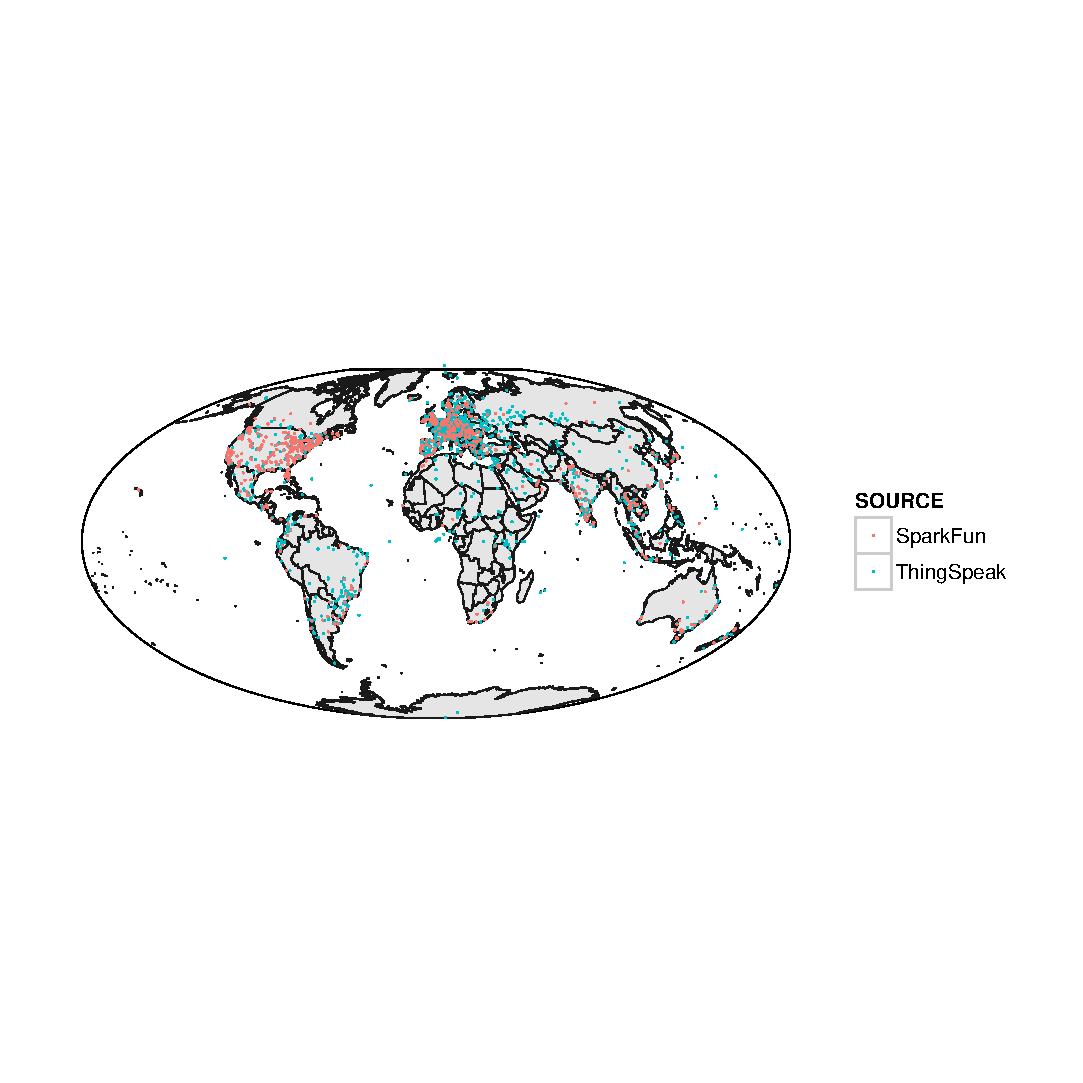
\includegraphics[width=0.65\textwidth]{img/map.eps} 
\caption{Location of all ThingSpeak and SparkFun sensing sources.}
\label{geo}
\end{figure*}

From such results it is clear the importance of information fusion from different sources, since not only the sampling number of the sensing infrastructure is incremented, but also its coverage.
Indeed, ThingSpeak appears to have much more utilization in the european region, whereas SparkFun seems to be more popular in North America.
Furthermore, this consideration might be extended to different macro topic areas, meaning that some open data sources are specialized on a specific field of measuring.
For instance, governmental sources providing open data such as EPA (United States Environmental Protection Agency) \cite{epa} are primarily focused on environmental data, whilst crowdsensing sources such as OpenSignal \cite{opensignal} regard measurements on cellular network signal strength and coverage.
\\

Raw data streams also provide temporal information, especially regarding the creation date and the last update date.
Such data can tell us much about the general trend in the usage of these platforms throughout a time window of few years.
Each stream in ThingSpeak comes with a creation date, which we reported in the diagram in figure~\ref{creationtrend}.
\begin{figure}[!t]
\centering
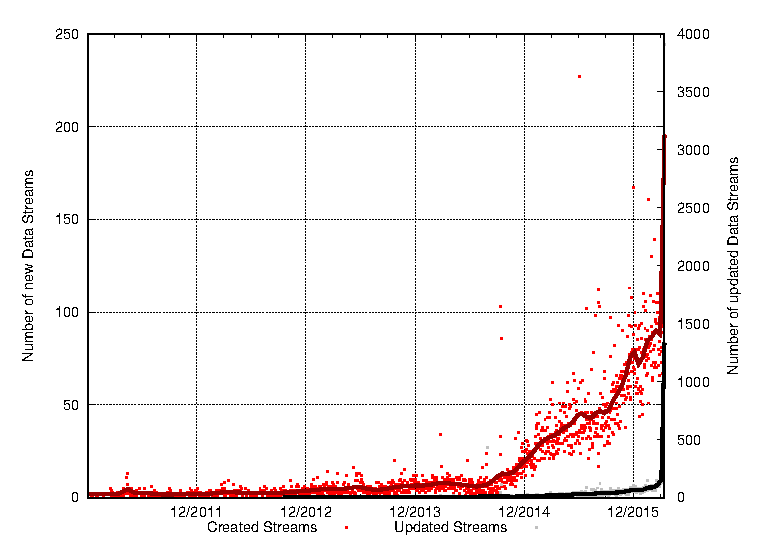
\includegraphics[width=0.50\textwidth]{img/bars.eps} 
\caption{Trend in creation of ThingSpeak channels.}
\label{creationtrend}
\end{figure}
From such analysis it results a substantial growth in created channels.
Some of the steeper slopes are probably justifiable.
A possible intuition behind them is the parallel innovation in simple hardware modules, for instance August 2014 corresponds to the launch of the first version of ESP8266 on the market and in October 2014 was possible to flash its firmware though an SDK \cite{espressif}.
Such period has not surprisingly been affected by a rapid growth according to the diagram.



\section{Data Unification}
\label{unification}

\section{Conclusions}





\bibliographystyle{IEEEtran}
% argument is your BibTeX string definitions and bibliography database(s)
\bibliography{bare_conf}
\end{document}          
